\chapter{Grundlagen}

\section{Data Mining Frameworks}
Wie in Abschnitt \ref{sec:DataMining} bereits erwähnt, haben sich um das Data Mining drei bekannte Frameworks entwickelt. Diese werden im Nachfolgenden genauer betrachtet. Anschließend findet die Auswahl statt, welches Rahmenwerk Anwendung in dieser Arbeit findet.

\subsection{Knowledge Discovery in Databases (KDD) process model}
Die Bezeichung Knowledge Discovery in Databases wurde hauptsächlich von \citep{fayyad_data_1996} geprägt. Sie beschreiben in ihrer Arbeit ein Problem der 1990er Jahre. Wie auch heute noch, stieg damals die Masse der gespeicherten Daten exponentiell \todo{wirklich "exponentiell"?} an. Die Manuelle Auswertung dieser Datensätze erforderte mehr Arbeitskraft als vorhanden war. \citep[S.~38]{fayyad_data_1996} beschreiben es als "data overload". Deswegen versuchte man, die Prozesse zur Findung von Erkenntnissen zu automatisieren. Daraus hat sich ein Standardvorgehen entwickelt, dass das KDD-Prozessmodell darstellt.
\begin{figure}[h]
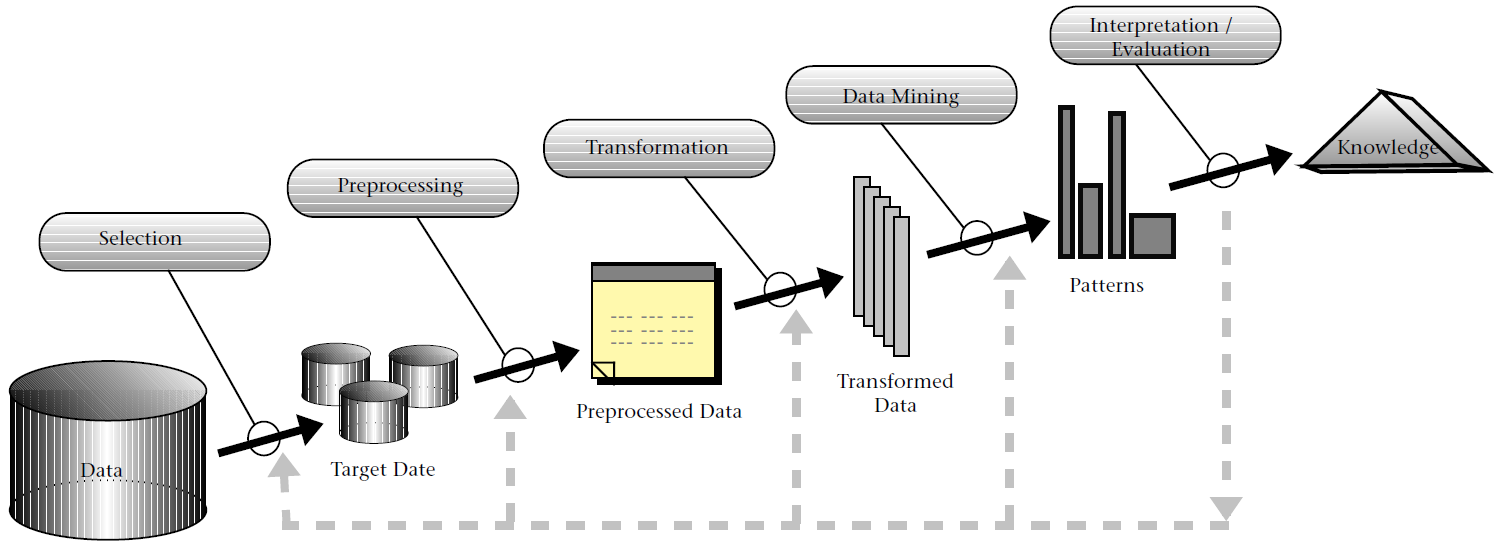
\includegraphics[width=\textwidth]{images/kddprocess}
\caption{Ein Überblick über die Schritte des KDD Prozesses nach \citep[S.~41]{fayyad_data_1996}}
\label{fig:kddprocess}
\centering
\end{figure}


\subsubsection{Selection}
Bevor der erste eigentliche Schritt, die Selektion der Daten, erfolgen kann, ist es unabdingbar, ein "Verständnis für das Anwendungsgebiet zu entwickeln".\citep[S.~42; eigene Übersetzung]{fayyad_data_1996} Dies inkludiert auch, Ziele zu setzen und Fragen zu formulieren, die durch das spätere Data Mining (Schritt \ref{subsubsec:DataMining}) beantwortet werden sollen. \todo{wirklich "Ziele setzten"?} Ist das Verständnis hergestellt, kann ein "target data set"\citep[S.~42]{fayyad_data_1996} hergestellt werden. Dabei werden zuerst Daten aus unterschiedlichen - oft heterogenen - Quellen zusammengeführt und dann hinsichtlich des Ziels verdichtet.\citep[S.~70]{swamynathan_mastering_2017}

\subsubsection{Preprocessing}
Die verbleibende Teilmenge der ursprünglichen Daten muss nun noch gesäubert und für die nächsten Schritte vorbereitet werden. Dies geschieht, da unbereinigte Daten sowohl den Data Mining-Prozess verschlechtern können (unverlässliche oder falsche Ergebnisse), als auch die Zeit für das Mining deutlich verlängern können.\citep[S.~70]{swamynathan_mastering_2017}
Um die Qualität der Daten und des Mining zu verbessern, werden unter anderem folgende Aspekte betrachtet:\multicitep{fayyad_data_1996, S.~42; swamynathan_mastering_2017, S.~70}
\paragraph{Outliner treatment}\mbox{} \\
Ein Ausreißer (engl. outliner) kann beispielsweise ein "Extremer Wert in einer Variablen" oder ein "Extremer Wert des Residuums bei einer sinnvollen Regression"\citep[S.~25; Teil 5b]{hertle_datenanalyse_2016} sein. Ein Vorgehen für Ausreißer kann folgendermaßen aussehen (nach \citep[S.~25; Teil 5b]{hertle_datenanalyse_2016}):
\begin{enumerate}
\item Identifizieren der Ausreißer (evtl. durch eine erste Regression)
\item Interpretation im Sachzusammenhang (Messfehler oder wichtiger Teil der Population)
\item Entscheidung, ob man eine Regression der Daten mit oder ohne diese Ausreißer haben möchte
\item In der Darstellung der Ergebnisse auf die Ausreißer explizit eingehen und Vorgehen erläutern
\end{enumerate}

\paragraph{Noise removal}\mbox{} \\
Auch in einem Datensatz, der auf Ausreißer untersucht wurde, befinden sich immer noch unbekannte, unvollständige, falsche und fehlende Werte ("attribute noise"). Zusätzlich können Datenklassen falsch gekennzeichnet sein ("class noise"). Ist ein Datensatz von diesen Problemen betroffen, spricht man von "noisy data". Auf die Lösung dieses Problems wird an dieser Stelle nicht weiter eingegangen. 

\paragraph{Identifying duplicated values}\mbox{} \\
Wie oben angesprochen, wird der zu analysierende Datensatz aus mehreren Quellen zusammengeführt. Durch diesen Schritt können Datensätze doppelt (oder noch öfter) vorkommen. Das wird deutlich, wenn man folgendes Beispiel betrachtet: \newline
Über eine Kundenkarte werden Daten von Kunden eines Supermarkets je Filiale gespeichert. Bei einer überregionalen Kundenanalyse tauchen Kunden mehrfach auf, die in verschiedenen Filialen eingekauft haben. Hier ist anzumerken, dass doppelte Werte nicht zwangsläufig gelöscht werden müssen, sie sollten jedoch bei der Analyse bedacht werden.

\paragraph{Check for inconsistency}\mbox{} \\
Je größer ein Datensatz ist, umso wahrscheinlicher enthält der auch Inkonsistenzen \todo{quelle hierfür?}. Dies wird ebenfalls durch die Fusion von mehreren Quellen verstärkt (Beispiel: unterschiedliches Alter für einen Kundenstammsatz). Auch hier muss geprüft werden, wie mit diesen Werten umzugehen ist. Eventuell können Regeln festgelegt werden wie "immer der neuste Datenpunk ist der richtige".

\paragraph{Time series and changes}\mbox{} \\
Der letzte Punkt, der beim Preprocessing betrachtet werden muss, ist der Zusammenhang der Daten und dem Erfassungszeitpunkt. So können sich im Laufe der Zeit die Messmethodik (z.B. andere Sensoren), die Messgenauigkeit (z.B. bessere Sensoren) oder die Abstände der Messungen verändern. \todo{warum ist das schlecht: ungleich verteilte Datensätze/inkonsistente Genauigkeit}

\subsubsection{Transformation}
Der letzte Schritt vor dem eigentlichen Data Mining ist die Transformation. In diesem Prozessschritt geht es darum, "mit Dimensionsreduktions- oder -transformationsmethonden die effektive Anzahl an Variablen [...] zu reduzieren"\citep[S.~42; eigene Übersetzung]{fayyad_data_1996}. Dies geschieht beispielsweise durch das identifizieren und eliminieren invarianter Variablen. Ebenfalls wird versucht, solche Variablen zu finden, die mehrere Andere repräsentieren. Anschaulich dargestellt an einem Beispiel:\newline
\begin{table}[h!]
\begin{tabular}{rrrrrrr}
  \hline
 & Person & Studium & ErfahrungExtern & ErfahrungIntern & Alter & Gehalt \\ 
  \hline
1 &   1 &   6 &   1 &   4 &  24 & 46450 \\ 
  2 &   2 &  18 &  30 &  15 &  55 & 85150 \\ 
  3 &   3 &  11 &   7 &   7 &  31 & 55900 \\ 
  4 &   4 &  11 &  15 &   8 &  36 & 63650 \\ 
  5 &   5 &  10 &   1 &  16 &  33 & 59050 \\ 
  6 &   6 &   6 &  25 &   6 &  38 & 68750 \\ 
  7 &   7 &  10 &  20 &  20 &  50 & 79000 \\ 
  8 &   8 &   7 &   0 &   1 &  23 & 43050 \\ 
   \hline
\end{tabular}
\caption{Einfacher Datensatz mit Berufserfahrung und Gehalt}
\label{tab:Beispiel_Berufserfahrung_R_output_simpleData}
\end{table}
Tabelle \ref{tab:Beispiel_Berufserfahrung_R_output_simpleData} zeigt einen einfachen Datensatz, in dem die Mitarbeiter einer Firma und die zugehörigen Gehälter festgehalten sind. "Studium" beschreibt die Anzahl der Halbjahre im Studium. Analog dazu "ErfahrungExtern" und "ErfahrungIntern" die Berufserfahrung in Halbjahren außerhalb und innerhalb der Firma. Zusätzlich ist das Alter der Personen gegeben.\newline
Führt man eine Regression (Listing \ref{list:Regression1}) für den Datensatz durch (mit Studium, ErfahrungExtern, ErfahrungIntern, Alter als unabhängige und Gehalt als abhängige Variablen), ergibt sich das Ergebnis in Tabelle \ref{tab:Regression1:output}.

\lstinputlisting[caption=Regression mit allen Faktoren,label=list:Regression1]{../R/Beispiel_Berufserfahrung/Regression1.R}

\begin{table}[h!]
\begin{tabular}{rrrrr}
  \hline
 & Estimate & Std. Error & t value & Pr($>$||) \\ 
  \hline
(Intercept) & 40000 & 1.415e-11 & 2.828e+15 & <2e-16 *** \\ 
  Studium & 300 & 5.167e-13 & 5.807e+14 & <2e-16 *** \\ 
  ErfahrungExtern & 850 & 4.821e-13 & 1.763e+15  & <2e-16 *** \\ 
  ErfahrungIntern & 950 & 6.308e-13 & 1.506e+15 & <2e-16 *** \\ 
  Alter & 2.010e-13 & 8.103e-13 & 2.480e-01 & 0.82 \\ 
\hline
\end{tabular}
\caption{Output der Regression mit allen Variablen}
\label{tab:Regression1:output}
\end{table}

Ohne weiter auf die genauen Beizeichnungen einzugehen, gibt die Sternnotation von R an, dass die unabhängigen Variablen Studium, ErfahrungIntern und ErfahrungExtern signifikant sind. Das Alter hingegen nicht. Die Regression hat ein adjustiertes Bestimmtheitsmaß ($R^2$; engl. adjusted R-squared) von 1. Das Bedeutet, dass das Gehalt vollständig durch die gegebenen Variablen erklärt werden kann (dies wird in der Realität jedoch nie erreicht).

\lstinputlisting[caption=Regression ohne Alter,label=list:Regression2]{../R/Beispiel_Berufserfahrung/Regression2.R}
\begin{table}[h!]
\begin{tabular}{rrrrr}
  \hline
 & Estimate & Std. Error & t value & Pr($>$||) \\ 
  \hline
(Intercept) & 40000 & 2.393e-12 & 1.671e+16 & <2e-16 *** \\ 
  Studium & 300 & 2.948e-13 & 1.018e+15 & <2e-16 *** \\ 
  ErfahrungExtern & 850 & 8.948e-14 & 9.500e+15 & <2e-16 *** \\ 
  ErfahrungIntern & 950 & 1.642e-13 & 5.787e+15.75 & <2e-16 *** \\ 
\hline
\end{tabular}
\caption{Output der Regression ohne Alters-Variable}
\label{tab:Regression2:output}
\end{table}
Führt man die Regression nun ohne das Alter durch (Listing \ref{list:Regression2} und Tabelle \ref{tab:Regression2:output}) bleibt $R^2$ gleich. Der Datensatz wurde also bereits um eine Variable reduziert, ohne das Ergebnis der Regression zu verschlechtern.\newline
Betrachtet man die Faktoren ErfahrungExtern und ErfahrungIntern, so fällt auf, dass sie einen ähnlichen Einfluss auf das Gehalte erzielen (850 und 950). 
\lstinputlisting[caption=Regression mit zusammengefassten Werten,label=list:Regression3]{../R/Beispiel_Berufserfahrung/Regression3.R}
Fasst man beide Variablen zusammen (Listing \ref{list:Regression3}), zeigt sich im Ergebnis (Tabelle \ref{tab:Regression3:output}), dass $R^2$ bei 0,9988 liegt. Die Güte der Regression hat sich also nur minimal verschlechtert.
\begin{table}[h!]
\begin{tabular}{rrrrr}
  \hline
 & Estimate & Std. Error & t value & Pr($>$||) \\ 
  \hline
(Intercept) & 40107.10 & 528.87 & 75.83 & 7.55e-09 *** \\
ErfahrungGesamt & 876.69 & 15.86 & 55.26 & 3.67e-08 ***\\ 
Studium & 327.17 & 64.27 & 5.09 & 0.0038 **\\ 
\hline
\end{tabular}
\caption{Output der Regression mit zusammengefassten Werten}
\label{tab:Regression3:output}
\end{table}
Zusammenfassend lässt sich für dieses Beispiel sagen, dass die Variablen im Datensatz um die Hälfte reduziert wurden, ohne die Aussagekraft deutlich zu verschlechtern. In einem realen Datensatz ist diese Arbeit zwar nicht so trivial und offensichtlich, jedoch gelten die gleichen Prinzipien.\newline
Nach \citep[S.~71; veränderte Version]{swamynathan_mastering_2017} gibt es zur Transformation folgende Möglichkeiten:
\begin{itemize}
\item Smoothing (binning, clustering, regression, etc.)
\item Aggregation (im Beispiel: das Zusammenfassen der Berufserfahrung)
\item Generalization (Ersetzen von primitiven Datenobjekten durch höherstufige Konzepte)
\item Normalization (min-max-scaling oder z-score)
\item Feature construction aus bereits bestehenden Attributen durch Techniken wie die Hauptkomponentenanalyse (engl. principal components analysis; PCA), Multidimensional scaling (MDS) oder Locally-linear embedding (LLE)
\item Compression (zum Beispiel wavelets, PCA, clustering etc.)
\item andere Datenreduzierungstechniken bei denen das Datenvolumen sinkt, ohne die Integrität der Originaldaten zu verletzten
\end{itemize}


\subsubsection{Data Mining}\label{subsubsec:DataMining}
Ist der Datensatz präpariert, so findet das eigentliche Data Mining statt. Dabei muss sich der Anwender für eine oder auch mehrere Methoden für das Mining entscheiden, um die anfänglichen Ziele zu erreichen und die Fragestellungen zu beantworten. Zur Auswahl stehen beispielsweise\multicitep{fayyad_data_1996, S.~42; swamynathan_mastering_2017, S.~71}:
\begin{itemize}
\item zusammenfassende und beschreibende Methoden: Mittelwert (arithmetisches Mittel), Median, Modus, Standardabweichung, Klassen-und Konzeptbeschreibungen, grafische Plots,
\item Vorhersagende Modelle (engl. predictive models): Klassifikationen und Regressionen und
\item Cluster-Analysen.
\end{itemize}
Eine genauere Beschreibung der Methoden (und der zugehörigen Algorithmen) im Kontext des Machine Learning befindet sich in Abschnitt \ref{sec:MachineLearning}. Je nach Beschaffenheit der zugrundeliegenden Daten und der gewählten Methode, muss ein passender Algorithmus gewählt und dieser korrekt parametrisiert werden. Zum Data Mining gehört auch, Hypothesen zu formulieren und das Ergebnis im Auge zu behalten: Ist der Endnutzer der Analyse an einem vorhersagenden Model interessiert (zum Beispiel für Wartungsarbeiten) oder an einem Jetzt-bezogenen (zum Beispiel für eine strategische Ausrichtung nach den aktuellen Kundensegmenten)?\newline
Anschließend erfolgt das (automatische) Mining der Daten. Je besser die vorhergehenden Schritte durchgeführt wurden, desto potenter ist das Ergebnis.\citep[S.~42]{fayyad_data_1996} Aus diesem Grund ist es auch jederzeit möglich, zu einem vorangegangen Prozessschritt zu springen, um neu erlangte Einsichten einfließen zu lassen (siehe zurückspringender grauer Pfeil in Abbildung \ref{fig:kddprocess}).

\subsubsection{Interpretation/Evaluation}
Zuletzt werden die gefundenen Muster und trainierten Modelle interpretiert. Ein Muster macht Aussagen über jeden Datenpunkt im betrachteten Raum. Ein Beispiel bei einem einfachen linearen Model: $$y = m \times x + t$$
Zu obigem Fall: $$Gehalt = Studium \times 327,17 + ErfahrungGesamt \times 876,69 + 40107,10$$ Ein Muster (engl. pattern) beschreibt dagegen nur eine kleine "lokale Struktur", die "nur über einen begrenzen Bereich" Aussagen macht.\citep[S.~71; eigene Übersetzung]{swamynathan_mastering_2017} Im Fall des linearen Model, wäre es eine bestimmte Gleichung, zum Beispiel $$y = 2 \times x + 5$$ oder $$ 6 \times 327,17 + 5 \times 876,69 + 40107,10 =  46453,57$$\citep{kraker_towards_2013}. "Fayyad et al. benutzt patterns und models synonym".\citep{kraker_towards_2013}\newline
Das Interpretieren der Ergebnisse beinhaltet ebenfalls das Zusammenfassen der Erkenntnisse und gegebenenfalls das Visualisieren.\citep[S.~71]{swamynathan_mastering_2017} Als Evaluieren wird das Eingliedern der Resultate in andere Systeme (zur Weiterverarbeitung oder Verbreitung), das Prüfen auf (und Lösen von) Konflikten mit anderen Untersuchungen und nicht zuletzt das Dokumentieren der Befunde bezeichnet.\citep[S.~42]{fayyad_data_1996} \newline
\todo{Befund nur medizinisch?; synonym)}
An dieser Stelle sei erneut angemerkt, dass das erste Ergebnis des KDD-Prozesses nicht das Endergebnis sein muss. Es kann durchaus viele Iterationen geben, die auch "loops between any two steps" beinhalten können.\citep[S.~42]{fayyad_data_1996}




\subsection{CRoss Industrial Standard Process for Data Mining (CRISP – DM)}
Bei CRoss Industrial Standard Process for Data Mining handelt es sich - wie bei KDD - um ein Referenzmodell für Data Mining. Das Modell wurde von einem 1996 gegründeten Konsortium aus "Daimler-Benz (now DaimlerChrysler), Integral Solutions Ltd. (ISL) [jetzt SPSS], NCR, and OHRA"\citep[S.~13]{shearer_crisp-dm_2000} erarbeitet. Die Version 1.0 wurde 2000 vorgestellt.\citep[S.~13]{shearer_crisp-dm_2000} In Umfragen (1999, 2002, 2004, 2007) wird das Modell als führend in Bereich von "data mining/predictive analytics projects"\citep[S.~72]{swamynathan_mastering_2017} bezeichnet. Das Modell ist "nicht-properitär, dokumnetiert und frei verfügbar"\citep[S.~13; eigene Übersetzung]{shearer_crisp-dm_2000}. Es ist ebenfalls in vielen Bereichen nutzbar, da es weder Industriesektor-, Werkzeugs- noch Anwendungsspezifisch ist. Grundsätzlich bekräftigt das Modell best practices und soll zu besseren und schnelleren Ergebnissen führen.\citep[S.~13; eigene Übersetzung]{shearer_crisp-dm_2000} \todo{evtl. bessere Bezeichnung}\newline 


\begin{figure}[h]
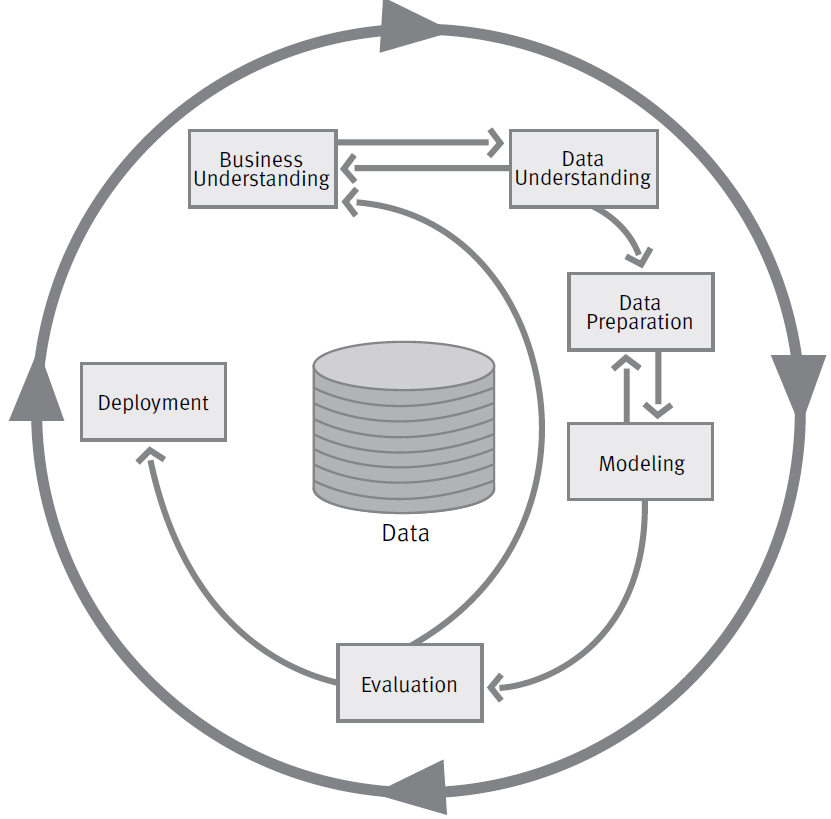
\includegraphics[width=\textwidth]{images/CRISP_DM}
\caption{Phasen des CRISP-DM Referenzmodells nach \citep[S.~10]{chapman_crisp-dm_2000}}
\label{fig:CRISP_DM}
\centering
\end{figure}

Wie in Abbildung \ref{fig:CRISP_DM} zu sehen ist, umfasst das Referenzmodell sechs Phasen. Genau wie beim KDD-Prozessmodell handelt es sich nicht um ein lineares Modell, sondern um eines, das Rückschritte und Iterationen erlaubt. Im Nachfolgenden werden die Prozessschritte und ihre Unterschritte kurz vorgestellt. Als Referenz dient unter anderem Abbildung \ref{fig:CRISP_DM_detailed}, die zusätzlich den Output der einzelnen Schritte zeigt.

\begin{figure}[h]
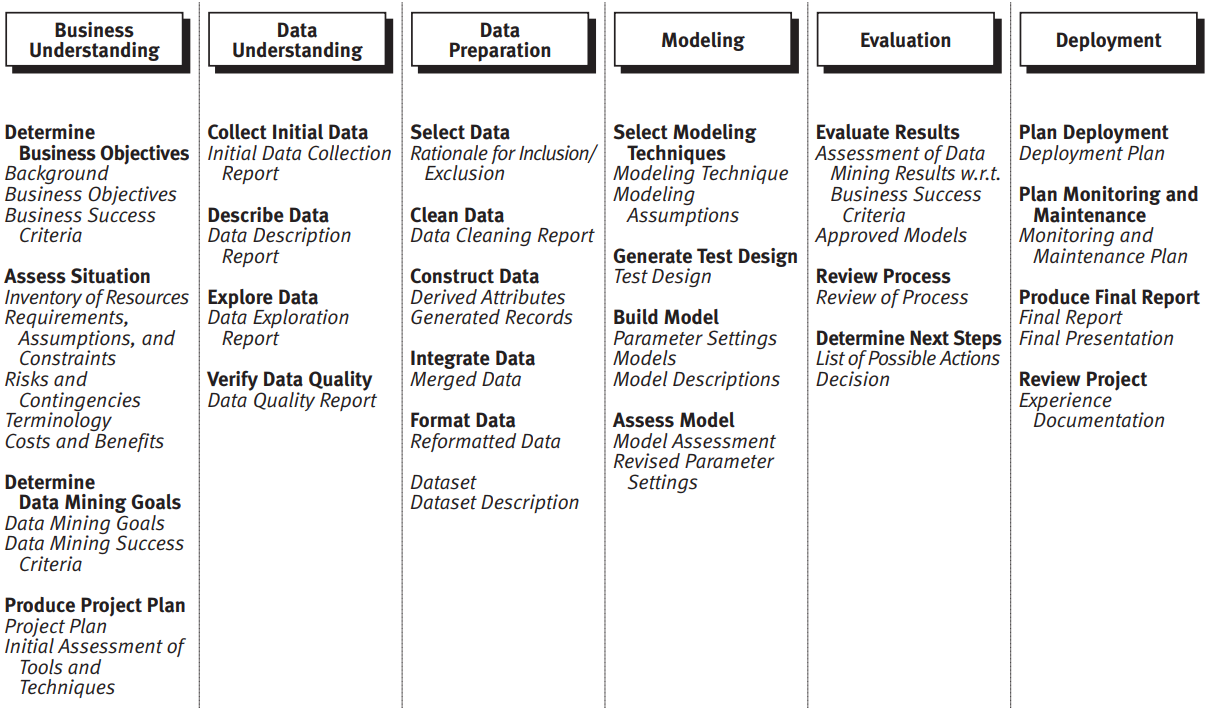
\includegraphics[width=\textwidth]{images/crisp_dm_detailed}
\caption{Generische Aufgaben (bold) und Output (italic) des CRISP-DM Referenzmodells \citep[S.~12]{chapman_crisp-dm_2000}}
\label{fig:CRISP_DM_detailed}
\centering
\end{figure}

\subsubsection{Business Understanding}
Die erste und vielleicht wichtigste Phase\citep[S.~14]{shearer_crisp-dm_2000} des CRISP-DM Prozesses ist das "Business Understandin", oder auch "Research Understanding"\citep[Punkt 1.4.1.1]{larose_discovering_2014}. Die Aufgabe dieser Phase ist, die "Ziele und Erwartungen"\citep[S.~73]{swamynathan_mastering_2017} des Projektes zu verstehen, dieses "Wissen in eine Machine Learning Problem Definition zu übersetzen" und schließlich einen "Vorläufigen Plan"\citep[S.~14]{shearer_crisp-dm_2000} aufzustellen. 
\paragraph{Determine the Business Objectives}\mbox{} \\
Dieser Teilschritt soll hauptsächlich die Frage beantworten, warum die Analyse durchgeführt wird. Dies hat direkten Einfluss auf die Zeile des Projekts und soll verhindern, dass "viel Aufwand für das Finden von richtigen Antworten auf die falschen Fragen"\citep[S.~14]{chapman_crisp-dm_2000} verschwendet wird.
\paragraph{Assess the Situation}\mbox{} \\
Um das Ziel der Analyse so genau wie möglich zu treffen, muss genau nachgeforscht werden, welche Ressourcen verfügbar sind, welchen Zwängen und Grenzen die Analyse unterlegen ist und unter welchen Annahmen sie stattfindet.\citep[S.~14]{chapman_crisp-dm_2000} Vereinfacht lässt sich sagen, dass hier die Fragen aus dem vorhergehenden Schritt detaillierter betrachtet werden.
\paragraph{Determine the Data Mining Goals}\mbox{} \\
Die gefundenen Ziele sind meist in Geschäftssprache formuliert. Für die Analyse müssen die Ziele jedoch im Terminus technicus des Data Mining formuliert sein. Ein Beispiel dazu ist die Übersetzung von "Increase catalog sales to existing customers." in "Predict how many widgets a customer will buy, given their purchases over the
past three years, demographic information (age, salary, city, etc.), and the price of the item."\citep[S.~16]{chapman_crisp-dm_2000}

\paragraph{Produce a Project Plan}\mbox{} \\

\subsubsection{Data Understanding}

\paragraph{Collect the Initial Data}\mbox{} \\
\paragraph{Describe the Data}\mbox{} \\
\paragraph{Explore the Data}\mbox{} \\
\paragraph{Verify Data Quality}\mbox{} \\
\subsubsection{Data Preparation}
\paragraph{Select Data}\mbox{} \\
\paragraph{Clean Data}\mbox{} \\
\paragraph{Construct Data}\mbox{} \\
\paragraph{Integrate Data}\mbox{} \\
\paragraph{Format Data}\mbox{} \\
\subsubsection{Modeling}
\paragraph{Select the Modeling Technique}\mbox{} \\
\paragraph{Generate Test Design}\mbox{} \\
\paragraph{Build the Model}\mbox{} \\
\paragraph{Assess the Model}\mbox{} \\


\subsubsection{Evaluation}
\paragraph{Evaluate Results}\mbox{} \\
\paragraph{Review Process}\mbox{} \\
\paragraph{Determine Next Steps}\mbox{} \\

\subsubsection{Deployment}
\paragraph{Plan Deployment}\mbox{} \\
\paragraph{Plan Monitoring and Maintenance}\mbox{} \\
\paragraph{Produce Final Report}\mbox{} \\
\paragraph{Review Project}\mbox{} \\

\subsection{Sample, Explore, Modify, Model and Assess (SEMMA)}
\subsection{Auswahl}


\section{Machine Learning}\label{sec:MachineLearning} 

\todo{semi supervised etc.}
\subsection{Supervised...}
Man weiß, nach was man sucht…
\subsubsection{Decision Tree}
\subsubsection{Neares Neighbour}
\subsubsection{Random Forest}
\subsubsection{SVM}
\subsection{Unsupervised...}
\subsubsection{K means}
\subsubsection{Hierarchical clustering}
\subsubsection{Neuronal networks}
\subsubsection{...}
Man sucht nur cluster/gruppen/etc




\section{Krypotwährung(en)}
Bitcoin,ethereum, litecoin, dogecoin; auswahl hier nur 1/2


\section{SaaS}
\section{Microsoft Azure ML Studio}
\subsection{Allgemeine Beschreibung}
\subsection{Aufbau }
\subsubsection{Projects}
\subsubsection{Experiments}
\subsubsection{Web Services}
\subsubsection{Notebooks}
\subsubsection{Datasets}
\subsubsection{Trained Models}
\subsubsection{Settings}
\subsection{Elemente}
relevate auswählen
\subsubsection{Saved Datasets}
\subsubsection{Data Transformation Conversations}
\subsubsection{Data Transformation}
\subsubsection{Data Input and Output}
\subsubsection{Feature Selection}
\subsubsection{Machine Learning}
\subsubsection{OpenCV Library Models}
\subsubsection{Python Language Model}
\subsubsection{R Language Model}
\subsubsection{Statistical Functions}
\subsubsection{Text Analysis}
\subsubsection{Time Series Anomaly Detection}
\subsubsection{Web Service}
